\chapter{Generating surfaces and fractures\label{chap:generating_surfaces}}
% \hl{Stuff to define?}
% \begin{itemize}
%     \item fBm surfaces
%     \item Hurst exponent
%     \item Gaussian random variable ?
%     \item non-stationary
%     \item self-similar
%     \item isotropic
%     \item lacunarity
% \end{itemize}

\todobo{More introduction to generating surfaces?}
% When generating random surfaces we want to be able to control the properties like the Hurst exponent (\hl{etc.?}) of the surface.

To generate random surfaces we use an iterative midpoint displacement method usually called successive random additions (SRA). The method is based on a method proposed by Fourner in 1982\cite{fournier1982computer}, but with some modifications suggested by Voss\cite{voss1985random, voss1988fractals}. The method has further been discussed by Saupe\cite{saupe1988algorithms}, amongst others. We choose this method mainly because it is possible to generate periodic surfaces with it, because it generates very good approximations to fBm surfaces\cite{zhou2005comparison}, and because the Hurst exponent of the generated surfaces is easy to control. The method is also easy to understand, easy to implement, and generates surfaces with high resolution very fast. The method is widely used in scientific applications because of these properties, and is also used for generating surfaces in computer graphics, since the surfaces look very realistic.

\section{Midpoint displacement methods}
% \todo[inline]{The most basic method we used is a very basic but widely used method, which has many variations and names. The most common names are ``the diamond-square algorithm''\hl{cite}, ``the midpoint displacement method''\hl{cite}, ``plasma fractal'' and ``cloud fractal''.}
%
The method we use to generate random surfaces is very similar to the standard midpoint displacement method (MDM), so we start with showing that method. In 1 dimension this method goes as follows
%
\begin{enumerate}
    \item Give the values at the endpoints of the interval, $y_0$ and $y_n$, random values from a Gaussian random variable with mean $\mu = 0$ and variance $\sigma_0^2$. This initial standard deviation $\sigma_0$ can be chosen freely.
    \item Generate the value in the center of the interval, $y_{n/2}$, by averaging over the two endpoints and adding a Gaussian random number with mean $\mu = 0$ and a \emph{reduced} variance
    \begin{align}
         \sigma_1^2 = \left(1/2\right)^{2H}\sigma_0^2, \label{eq:midpoint_sigma_first}
    \end{align}
    where $H$ is the wanted Hurst exponent.
    \item Continue generating the values in the center of each sub-interval until you reach the desired number of points, while reducing the variance of the random number by a factor $\frac{1}{2}$ each iteration. %
    %\todo{Why 1/2? (needed to create good approx. to fBm, see \cite{voss1985random})}. %
    For iteration $i$ we have
    \begin{align}
        \sigma_i^2 = \left(1/2\right)^{i2H}\sigma_0^2. \label{eq:midpoint_sigma_general}
    \end{align}
\end{enumerate}
%
\begin{figure}[htpb]%
    \centering%
    \includesvg[pretex=\small, width=0.5\textwidth, svgpath=./images/diamond_square/]{random_midpoint_displacement_regular02}%
    \caption{%
        Illustration of the midpoint displacement method in 1 dimension. We increase the number of points from 2 to 9 using 3 iterations.%
        \label{fig:midpoint01}%
    }%
\end{figure}%
See \cref{fig:midpoint01} for a visual illustration of the method.

This method generates a 1-dimensional line, with a Hurst exponent to the input $H$. But since we only add random numbers to the \emph{new} values we generate each iteration, the result is non-stationary for $H \neq 0.5$\cite{voss1985random}, and it is neither truly self-similar or isotropic, as noted by Mandelbrot\cite{mandelbrot1982comment}. To mitigate this we implement the addition suggested by Voss\cite{voss1985random}, which consists of adding a random number to \emph{all} points in each iteration, both the new and old. Voss called this modified method \emph{successive random additions}. %\todobo{Remove this last part, or make relevant?}

\section{Successive random additions}
The method called \emph{successive random additions} (SRA) is a modification of the regular midpoint displacement method first described by Richard F. Voss in \cite{voss1985random}, where we add random numbers to \emph{all} points in each iteration, compared to just adding random numbers to the \emph{new} points in the regular midpoint displacement method. This modification means that we can replace the factor $(1/2)$ in \cref{eq:midpoint_sigma_first,eq:midpoint_sigma_general} with a general parameter $r$,%
%\todoco{why? (something about distance between points)}% 
and we get the following variance for iteration $i$
\begin{align*}
    \sigma_i^2 = r^{2H}\sigma^2_{i-1}.
\end{align*}
This new parameter $r$ controls the lacunarity of the surface, without affecting the Hurst exponent.%
\todoco{Define lacunarity? - defined by equation above..}
% \hl{$r$ controls the lacunarity/roughness, $H$ independent of $r$}

% \subsection{(on an infinite grid) in 2 dimensions}
\subsection{Infinite grids}
Voss has geneneralized the the method of successive random additions to higher dimensions\cite{voss1985random}, and this generalized form is the algorithm we use when generating fractures. We use the method to generate surfaces in the form of heightmaps, meaning a 2-dimensional grid of points ({$i,j$}), with a value for the height in each point, $z(i,j) = z_{i,j}$, which is generated by the algorithm.

The central part of the algorithm consists of two steps often called the \emph{diamond-step} and the \emph{square-step}. We start with a simple case of an infinite grid of evenly spaced points, all with known $z$-values. The two steps are as follows:
\begin{description}
    \item[The \emph{square-step}:] The grid can be divided into small squares consisting of four points in each square, as in the leftmost square in \cref{fig:simple_square_step}. We generate the $z$-value in the center of each of these squares by averaging the $z$-values of the four corners of each square, as indicated by the red dots and arrows in \cref{fig:simple_square_step}. Then add a random Gaussian number with mean $\mu = 0$ and variance $\sigma_n^2 = \sigma_{n-1}^2r^{2H}$ to all new and old points, where $\sigma_{n-1}^2$ is the variance used in the previous step of the algorithm.
    \label{enum:test}
    
    \item[The \emph{diamond-step}:] After the square-step the grid can be divided into smaller squares that are tilted by 45 degrees, as in the leftmost square in \cref{fig:simple_diamond_step}. We generate the $z$-values in the center of each square by averaging the $z$-values of the four corners of each square, as indicated by the red dots and arrows in \cref{fig:simple_diamond_step}. We then add a random Gaussian number with mean $\mu = 0$ and variance $\sigma_{n+1}^2 = \sigma_n^2r^{2H}$, to all new and old points. 
\end{description}
See \cref{fig:diamond_square_applied} for an illustration of the square-step and diamond-step applied once on a larger grid. 

\begin{figure}[htpb]%
\centering%
%
\setlength{\myfigwidth}{0.7\textwidth}%
\setlength{\mycaptionwidth}{0.3\textwidth}%
%
% \parbox[c][2cm][c]{\myfigwidth}{
%     \includesvg[width=\myfigwidth, svgpath = images/diamond_square/]{simple_square_step_solarized08}
% }
% \parbox[c][2cm][c]{\mycaptionwidth}{
%     \subcaption{Square-step}
%     \label{fig:simple_square_step}
% }
%
% \begin{minipage}[c][2cm][c]{\myfigwidth}
%     \includesvg[height=2cm, svgpath = images/diamond_square/]{simple_square_step_solarized08}
% \end{minipage}
% \begin{minipage}[c][2cm][c]{\mycaptionwidth}
%     \subcaption{Square-step}
%     \label{fig:simple_square_step}
% \end{minipage}
%
\begin{minipage}[c]{\myfigwidth}%
    \includesvg[width=\textwidth, svgpath = images/diamond_square/]{simple_square_step_solarized10}%
\end{minipage}%
\begin{minipage}[c]{\mycaptionwidth}%
    \subcaption{Square-step}%
    \label{fig:simple_square_step}%
\end{minipage}%
\\%
\vspace{2mm}%
\begin{minipage}[c]{\myfigwidth}%
    \includesvg[width=\textwidth, svgpath = images/diamond_square/]{simple_diamond_step_solarized07}%
\end{minipage}%
\begin{minipage}[c]{\mycaptionwidth}%
    \subcaption{Diamond-step}%
    \label{fig:simple_diamond_step}%
\end{minipage}%
%
\caption{Illustration of the two steps used in the diamond square algorithm for generating random surfaces. The grey points are old points, the black points are new points, and the red points are the points used in the calcuation of the averages when generating the new points.}%
\label{fig:diamond_square_steps}%
\end{figure}%

We see that by first applying the square-step and then applying the diamond-step, we add one point in between each point in each direction, almost doubling the resolution of the grid. In general we go from $N$ to $N + (N-1)$ points in each direction. By applying the algorithm several times we get
\begin{align}
    N_1 &= N_0 + (N_0-1) = 2N - 1 \nonumber\\
    N_2 &= 2N_1 - 1 = 4N_0 - 3 \nonumber\\
    N_3 &= 2N_2 - 1 = 9N_0 - 7 \nonumber\\
    &\vdotswithin{=} \nonumber\\
%     &\shortvdotswithin{=}
    N_n &= 2^n(N_0-1) + 1, \label{eq:diamond_step_resolution}
\end{align}
where $n$ is the number of times we have applied the algorithm, and $N$ is the number of points in each direction. This means that using the diamond-square algorithm we can go from any resolution $N_0$ to all resolutions satisfying $N_n = 2^n(N_0 - 1) + 1$, although if starting with points generated using a different method we do not have the same control over the Hurst exponent of the surface after generating new points.
%
\begin{figure}[htpb]%
    \centering%
    \includesvg[width=0.9\textwidth, svgpath = images/diamond_square/]{increase_resolution_solarized_starssquares04}%
    \caption{%
        The diamond-square algorithm applied once on a grid of $3\times 3$ points, increasing the number of points from 9 to 25. The orange square points are generated by the square-step (see \cref{fig:simple_square_step}), and the blue star-shaped points by the diamond-step (see \cref{fig:simple_diamond_step}).%
    }%
    \label{fig:diamond_square_applied}%
\end{figure}%

% \subsection{Successive random additions on a finite grid (in 2 dimensions)}
\subsection{Finite size effects\label{sec:diamond_square_2d_finite}}
Since we are using computers to generate our surfaces, which have limited memory, we can not use infinite grids. This means we get some special cases that needs to be taken care of when generating points near the edges of the grid.
%\tododo{transition to below}%

By applying the square step we generate one new point in the center of each square formed by the grid from the previous iteration, and in general we generate the $z$-values in the points
\begin{align}
%     &\left(i+1/2, j+1/2\right) &0\leq i,j < N_{n-1}, \label{eq:square_step_limits}
    &z(i+1/2, j+1/2) & i,j \in [0, N_{n-1}), \label{eq:square_step_limits}
\end{align}
where $(i,j)$ are the indices of the points in the grid after the previous iteration, and $N_{n-1}$ is the number of points in each direction in this grid. In general the averages we calculate for the new points can be written as
% \begin{align}
%     (x_{i+1/2}, y_{j+1/2}) 
%     &= \frac{1}{4}\big(
%         (x_i, y_j) + (x_{i+1}, y_j)\nonumber\\
%         &+ (x_i, y_{j+1}) + (x_{i+1}, y_{j+1})
%     \big)
%     &0\leq i,j < n.
%     \label{eq:square_step}
% \end{align}
\begin{align}
    z(i+1/2, j+1/2) 
    = \frac{1}{4}\Big[
        &z(i, j) + z(i+1, j) \nonumber\\
        &+ z(i, j+1) + z(i+1, j+1)
    \Big],
    \label{eq:square_step}
\end{align}
using the limits in \cref{eq:square_step_limits}. We see that the square-step only uses points inside the grid when calculating the averages, which means that we do not have to modify this step when going to a finite grid.

By applying the diamond-step we generate the values in the points
\begin{align}
    z(i+1/2, j) & &\text{for } & &i\in [0,N_{n-1}) & &\text{ and } & &j\in [0,N_{n-1}]& \label{eq:diamond_step_limits01} \\
    z(i, j+1/2) & &\text{for } & &i\in [0,N_{n-1}] & &\text{ and } & &j\in [0,N_{n-1})&, \label{eq:diamond_step_limits02}
\end{align}
and in general the averages we calculate for the new points can be written as
% \begin{align}
%     (x_{i+1/2}, y_j) 
%     &= 
%     \frac{1}{4}\big(
%         (x_i, y_j) + (x_{i+1}, y_j) + (x_{i+1/2}, y_{j-1/2}) + (x_{i+1/2}, y_{j+1/2})
%     \big) \label{eq:diamond_step01}\\
%     (x_i, y_{j+1/2}) 
%     &= 
%     \frac{1}{4}\big(
%         (x_i, y_j) + (x_i, y_{j+1}) + (x_{i-1/2}, y_{j+1/2}) + (x_{i+1/2}, y_{j+1/2})
%     \big). \label{eq:diamond_step02}
% \end{align}
\begin{align}
    z(i+1/2, j) 
    &= 
    \frac{1}{4}\Big[
        z(i, j) + z(i+1, j) \nonumber\\
        &\phantom{=\Big[}~~~%
            + z(i+1/2, j-1/2) + z(i+1/2, j+1/2)
    \Big]
    \label{eq:diamond_step01}\\
    z(i, j+1/2) 
    &= 
    \frac{1}{4}\Big[
        z(i,j) + z(i, j+1) \nonumber\\
        &\phantom{=\Big[}~~~%
            + z(i-1/2, j+1/2) + z(i+1/2, j+1/2)
    \Big],
    \label{eq:diamond_step02}
\end{align}
using the limits in \cref{eq:diamond_step_limits01,eq:diamond_step_limits02}. We find that when generating points near the edges of the surface using the diamond-step, specifically when generating the points along the top and bottom edge%
%\todobo{make these equations clearer?}%
%
\begin{align*} % LaTeX assumes that each equation consists of two parts separated by a &; also that each equation is separated from the one before by an &.
    &z(1/2, j) & &\text{and} & &z(n - 1/2, j) & &\text{for} & &j \in [0, N_{n-1}],
\end{align*}
and the points along the left and right edge
\begin{align*}
    &z(i, 1/2) & &\text{and} & &z(i, n - 1/2) & &\text{for} & &i \in [0, N_{n-1}],
\end{align*}
we need the values of points that lie outside the grid to calculate the averages. There are two possible solutions to this, that will generate different surfaces. If  we want to generate a periodic surface, the solution is to wrap around the edges using periodic boundary conditions, and find the point we need on the opposite side of the grid. For example (using $i = j = 0$)
\begin{align*}
    z(1/2, -1/2) &\rightarrow z(1/2, n-1/2). \\
    z(1/2, -1/2) &\rightarrow z(1/2, n-1/2)
\end{align*}
If generating a non-periodic surface we simply ignore the points that lie outside the grid when calculating the averages, and just calculate the average of the three other points.

% \subsection{Implementing successive random additions (on a finite grid in 2 dimensions)}
\subsection{Implementation\label{subsec:SRA_implementation}}
In our implementation we generate a surface on a finite grid of size $N\times N$, starting with only the $z$-values in the four corners defined, giving a resolution $N_0 = 2$. As shown in \cref{eq:diamond_step_resolution} the algorithm can go from any resolution $N_0$ to any resolution $N_p = 2^p(n_0-1) + 1$ by applying the algorithm $p$ times, which means that our implementation can generate surfaces with resolutions
\begin{align*}
    N &= 2^p(2-1) + 1 = 2^p + 1,
\end{align*}
where $p$ is any positive integer.

We implement generation of both periodic and non-periodic surfaces using using \crefrange{eq:square_step_limits}{eq:diamond_step02}, while skipping points outside the grid for non-periodic surfaces, and wrapping around the edges using periodic boundary conditions when generating periodic surfaces.

To ensure that the periodic surfaces actually turn out periodic we start with all four corners having the same value. We also let the right and bottom edge be equivalent to the left and top edge, respectively, which effectively means that all four corners should always have the same $z$-value. To ensure that the opposite edges stay equal to each other we never generate any points on the right and bottom edge, but just copy the $z$-values from the opposite edge after the diamond-step.

This leaves us with the following algorithm for generating a surface which approximates a 2-dimensional fractional Brownian motion with Hurst exponent $H$
\begin{enumerate}
    % \itemsep1pt \parskip0pt \parsep0pt
    \renewcommand{\labelitemii}{$\bullet$}
    
    \item Allocate a grid of size $N\times N$, where $N = 2^p + 1$, and $p$ is any positive integer. This grid will store the $z$-values, or the height of the surface, in each grid point $z(x,y)$.

    \item Initialize the $z$-values of the corners of the grid by drawing random numbers from a Gaussian distribution with mean $\mu = 0$ and variance $\sigma_0$. The initial variance can be chosen freely. The initial resolution is now $2\times 2$.
    \begin{itemize}
        \item If generating a periodic surface, give all four corners the same $z$-value.
    \end{itemize}
    
    \item Apply the square-step using \cref{eq:square_step_limits,eq:square_step}. Add a random Gaussian number with mean $\mu = 0$ and variance $\sigma_n = \sigma_{n-1}^2r^{2H}$ to all new and old points.
    \label{enum:square_step}

    \item Apply the diamond-step using \crefrange{eq:diamond_step01}{eq:diamond_step02}. Add a random Gaussian number with mean $\mu = 0$ and variance $\sigma_{n+1} = \sigma_n^2r^{2H}$ to all new and old points.
    \label{enum:diamond_step}
    
    \begin{itemize}
        \item If generating a periodic surface, skip generating $z$-values for points on the right and bottom edge using the diamond-step, and instead copy the values from the opposite edges after the diamond-step.
    \end{itemize}
    
    \item Repeat step \ref{enum:square_step} and \ref{enum:diamond_step} $p$ times until you reach the desired resolution of $N\times N$, where $N = 2^p + 1$. For step $n$ the variance of the random Gaussian numbers is
    \begin{align*}
        \sigma_n^2 = \sigma_0^2(r^n)^{2H}.
    \end{align*}
\end{enumerate}

We implement the method in \cpp, and make a \matlab\ interface to the \cpp-program, for fast visualization and testing. We implement both generation of periodic and non-periodic surfaces, and the midpoint displacement method, and successive random additions. 

See \cref{fig:diamond_square_surface} for a surface with resolution $33\times 33$ generated by the algorithm.%
%
% \begin{figure}[htpb]%
%     \centering%
%     \includesvg[width=0.7\textwidth, svgpath=./images/diamond_square/surface_example/]{surface_labels}%
%     \caption{%
%         Caption.%
%         \label{fig:diamond_square_surface}%
%     }%
% \end{figure}%
\begin{figure}[htpb]%
    \centering%
    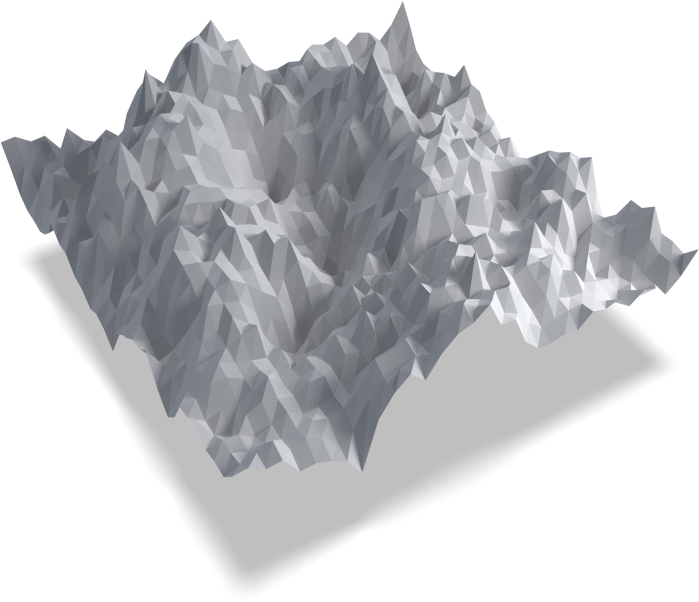
\includegraphics[width=0.5\textwidth]{./images/diamond_square/surface_blender/surface_composite01_cropped.png}%
    \caption{%
        A surface with resolution $33\times 33$ created using the midpoint displacement method called successive random additions.%
        \label{fig:diamond_square_surface}%
    }%
\end{figure}%
%
% \orangebox{
% {\bf Notes:}
% \begin{itemize}
%     \item Implementation (in Matlab/C++)?
%     \item periodic and non-periodic
%     \item Mention that DS can be used to increase resolution of any surface
%     \item Can increase resolution of generated surface, if we know the seed
% \end{itemize}
% 
% {\bf Stuff to define:}
% \begin{itemize}
%     \item Periodic/non-periodic
%     \item Lacunarity
% \end{itemize}
% }

\subsection[Validation and examples]{Validation \hl{and examples?}}
\todoao{Write more about testing diamondsquare/SRA}%
\todobo{colormap plot from above of surface?}%
To test the method for generating random surfaces, and to check that the Hurst exponent of the surfaces correspond to the wanted exponent, we generate surfaces and measure the Hurst exponent using the detrending moving average method from \cref{sec:dma}. We have implemented both the midpoint displacement method and successive random additions for generating random surfaces, both for periodic and non-periodic surfaces. A plot of the measured Hurst exponent (using DMA) as function of the input Hurst exponent can be seen in \cref{fig:diamond_square_testing}.%
%
\begin{figure}[!htb]%
    \centering%
    {
        \newcommand{\f}{\footnotesize}%
        \newcommand{\x}{\text}%
        \newcommand{\hh}{{\f $H_\x{in}=H_\x{out}$}}%
        \includesvg[width=0.7\textwidth, svgpath=./images/diamond_square_Hurst/test_diamondSquare/]{fig06}%
    }
    %
    % ---- Footnotemark in caption, and footnotetext below ---- %
    \caption[%
        Plot of the Hurst exponent measured using detrending moving average (DMA), as function of the input Hurst exponent to the synthesizing method. The dashed grey line indicates a measured Hurst exponent of 0.75, the solid grey line a measured exponent exactly equal to the input exponent ($H_\text{in} = H_\text{out}$). The green lines are for surfaces created using periodic boundary conditions (PBC), the red lines using non-periodic boundaries, the dashed lines using successive random additions (SRA), and the solid lines using the regular midpoint displacement method (MDM). We used 100 samples for each point, and input Hurst exponents between 0 and 1.2 in steps of 0.1. We have plotted the standard deviation in each point for SRA with periodic boundary conditions, and the standard deviation is about the same for the other combinations. %
    ]{%
        Plot of the Hurst exponent measured using detrending moving average (DMA), as function of the input Hurst exponent to the synthesizing method. The dashed grey line indicates a measured Hurst exponent of 0.75, the solid grey line a measured exponent exactly equal to the input exponent ($H_\text{in} = H_\text{out}$). The green lines are for surfaces created using periodic boundary conditions (PBC), the red lines using non-periodic boundaries, the dashed lines using successive random additions (SRA), and the solid lines using the regular midpoint displacement method (MDM). We used 100 samples for each point, and input Hurst exponents between 0 and 1.2\protect\footnotemark\ in steps of 0.1. We have plotted the standard deviation in each point for SRA with periodic boundary conditions, and the standard deviation is about the same for the other combinations. %
        \hl{FINISH CAPTION} %
        \label{fig:diamond_square_testing}%
    }%
%     %
%     % ---- Footnote in caption, and separate lof caption ---- %
%     \caption[%
%         Plot of the Hurst exponent measured using detrending moving average (DMA), as function of the input Hurst exponent to the synthesizing method. The dashed grey line indicates a measured Hurst exponent of 0.75, the solid grey line a measured exponent exactly equal to the input exponent ($H_\text{in} = H_\text{out}$). The green lines are for surfaces created using periodic boundary conditions (PBC), the red lines using non-periodic boundaries, the dashed lines using successive random additions (SRA), and the solid lines using the regular midpoint displacement method (MDM). We used 100 samples for each point, and input Hurst exponents between 0 and 1.2 in steps of 0.1. We have plotted the standard deviation in each point for SRA with periodic boundary conditions, and the standard deviation is about the same for the other combinations.%
%     ]{%
%         Plot of the Hurst exponent measured using detrending moving average (DMA), as function of the input Hurst exponent to the synthesizing method. The dashed grey line indicates a measured Hurst exponent of 0.75, the solid grey line a measured exponent exactly equal to the input exponent ($H_\text{in} = H_\text{out}$). The green lines are for surfaces created using periodic boundary conditions (PBC), the red lines using non-periodic boundaries, the dashed lines using successive random additions (SRA), and the solid lines using the regular midpoint displacement method (MDM). We used 100 samples for each point, and input Hurst exponents between 0 and 1.2\protect\footnote{test} in steps of 0.1. We have plotted the standard deviation in each point for SRA with periodic boundary conditions, and the standard deviation is about the same for the other combinations. %
%         \hl{FINISH CAPTION} %
%         \label{fig:diamond_square_testing}%
%     }%
\end{figure}%
\footnotetext{In reality we can not have Hurst exponents greater than 1, but as we see, the midpoint displacement methods generally creates surfaces with a measured exponent ($H_\text{out}$) lower than the input exponent ($H_\text{in}$) for $H_\text{in}>0.5$, so to we use some samples of $H_\text{in}>1$.}%

From the plot in \cref{fig:diamond_square_testing} we see that surfaces with periodic boundaries generally get a lower measured $H$ than non-periodic surfaces, at least for the surfaces with $H>0.5$. We also see that the surfaces generated using the midpoint displacement method (MDM) have very similar Hurst exponents as the ones generated using successive random additions (SRA). We see that the Hurst exponent of all surfaces is generally lower than the input exponent for input $H>0.5$, and lower than the input exponent for input $H<0.5$. We should take note of this when generating surfaces for our experiments, and make sure to measure the actual exponent, since we see that the standard deviation is relatively high.%
\todobo{Something about why periodic surfaces have lower exponent?}
